% Sandia National Laboratories is a multimission laboratory managed and
% operated by National Technology & Engineering Solutions of Sandia, LLC, a
% wholly owned subsidiary of Honeywell International Inc., for the U.S.
% Department of Energy’s National Nuclear Security Administration under
% contract DE-NA0003525.

% Copyright 2002-2019 National Technology & Engineering Solutions of Sandia,
% LLC (NTESS).

%%-------------------------------------------------------------------------
%% Purpose        : Main LaTeX Xyce Users' Guide
%% Special Notes  : Graphic files (pdf format) work with pdflatex.  To use
%%                  LaTeX, we need to use postcript versions.  Not sure why.
%% Creator        : Scott A. Hutchinson, Computational Sciences, SNL
%% Creation Date  : {05/23/2002}
%%
%%-------------------------------------------------------------------------

% -------------------------------------------------------------------------
% two level Analysis Chapter ----------------------------------------------
% -------------------------------------------------------------------------

\chapter{Handling Power Node Parasitics}
\label{PowerNode_Chap}
\index{two-level Newton}
\index{power node parasitics}

\chapteroverview{Chapter Overview}
{
This chapter includes the following sections:
\begin{XyceItemize}
\item Section~\ref{powerNode_Overview}, {\em Power Node Parasitics}
\item Section~\ref{twolevel_Overview}, {\em Two Level Algorithms Overview}
\item Section~\ref{twolevel_Examples}, {\em Examples}
\item Section~\ref{twolevel_restart}, {\em Restart}
\end{XyceItemize}
}

\section{Power Node Parasitics}
\label{powerNode_Overview}
\index{power node parasitics}

Parasitic elements (R, L, C) are frequently required for circuit simulations
to capture important circuit behavior.  Most parasitic elements 
(interconnects, etc.) can be added to netlists without causing any 
difficulties for the \Xyce{} solvers.   Small circuits in particular are
very robust to the addition of parasitic elements. Larger circuits, however, 
that must be simulated in parallel will in general tend to 
have more solver difficulties with the addition of parasitic devices.  
Of particular note are parasitic elements attached to the power and/or
ground nodes of large digital circuits.  An example of this is shown in
figure~\ref{powerNodeExample}.  As these nodes tend to be highly 
connected, they can potentially have a very high impact on solver difficulties.  

%  power node figure
\begin{figure}[b]
\vspace{-5pt}
  \centering
  \scalebox{0.40}
    {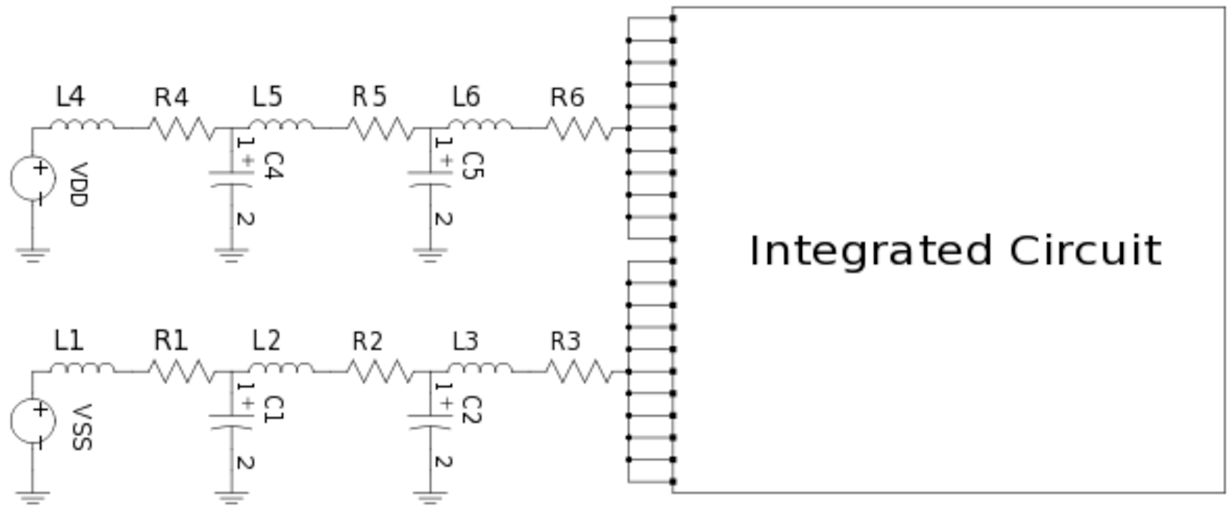
\includegraphics{paras_networkv2.pdf}}
\vspace{-5pt}
    \caption[Power node parasitics example.] {Power node parasitics example. 
NOTE:	An RLC network sits between the VDD, VSS sources and the main circuit, so these highly connected nodes cannot be removed with a singleton filter.}
    \label{powerNodeExample}
  \vspace{-10pt}
\end{figure}


One of the parallel algorithms used by \Xyce{} is called \emph{singleton 
removal}~\cite{ICCAD09_precond}, which is applied at the linear solver level and is crucial for getting many large circuits to run in parallel. This algorithm takes advantage of the fact that, in circuit simulation, some solution values are available explicitly, rather than being a quantity that needs to be calculated as the solution to a particular equation. In circuit simulation, such quantities are usually the values of independent sources. For instance, the presence of an independent voltage source at a particular node in a circuit fixes the voltage at that node to be the value of the independent source; therefore, equations reflecting the value of the voltage at that particular node do not have to be added to the set of linear equations used (in part) to determine the voltages at all the nodes in the circuit. The technique of fixing such node voltages without including them in the rest of the linear solve can be handled in a preprocessing phase referred to as the singleton removal phase.  

When simulating in parallel, singleton removal is crucial as some voltage 
sources (especially power supplies in digital circuits) are connected to 
hundreds or thousands of circuit nodes.  This presents a big 
problem in parallel because having numerous connections can often mean a communication 
bottleneck during the linear solve. Using singleton removal eliminates 
that bottleneck.

While singleton removal can result in a great improvement for circuits with 
ideal power supplies, for circuits with nonideal power supplies, the 
communication bottleneck remains.   Once parasitic elements 
are placed between the power supply and the rest of the circuit, it is only 
the voltage at the circuit node directly connected to the independent
source that can be removed via singleton removal.  Other nodes connected to this independent source through parasitic elements have 
voltages that must now be solved for directly.  


\section{Two Level Algorithms Overview}
\label{twolevel_Overview}

Fortunately, \Xyce{}~\cite{xyceBookChapter:2011} provides a workaround 
that allows power node parasitics to be included in large circuits without breaking singleton 
removal.  The workaround requires the use of a two-level Newton solve,
in which the problem is divided into two very separate pieces, each
for the most part treated as an entirely separate circuit with minimal coupling terms linking the pieces together.  

For power-node problems, two-level users will typically split the netlist 
into ''top'' and ''inner'' netlists.  The top netlist contains the
power node parasitics and the ideal voltage sources, and very little else.
The inner circuit should contain the rest of the circuit.  \Xyce{} couples the two
circuits through an ''EXT'' (external) device in the top circuit,
and two or more independent voltage sources on the inner circuit.  The
values on the inner voltages are imposed from the top circuit, and
the currents and conductances of the EXT device come from the inner
circuit.  An example is given below.

\Xyce{} will construct a different linear system for each circuit. As such, the inner circuit will appear to have independent sources, allowing the singleton removal algorithm to work.

Since at least the 1980s, literature has included the two-level Newton algorithm, although mostly as it applied to 
circuit-device simulation.  ~\cite{twolevelnewton} and~\cite{Mayaram2} provide a mathematical description, while ~\cite{xyceBookChapter:2011} provides more information about the \Xyce{} implementation.

\section{Examples}
\label{twolevel_Examples}

\begin{figure}[htbp]
\begin{centering}
\shadowbox{
\begin{minipage}{0.8\textwidth}
\begin{vquote}
THIS CIRCUIT IS THE TOP PART OF A TWO LEVEL EXAMPLE.
\color{blue}* compTop.cir - BSIM3 Transient Analysis\color{black}
\color{XyceRed}
YEXT y1 DD1 SS1 externcode=xyce netlist=compInner.cir \color{black}
Vdd DDorig 0 5.0
Vss SSorig 0 0.0

.options linsol type=klu
.options timeint abstol=1.0e-6  reltol=1.0e-3

\color{blue}* PARASITICS \color{black}
l\_Lwirevdd    DDorig Ny  .50n
l\_Lwirevss    SSorig Nx  .50n
R\_Rbw         Ny     DD1   50m
R\_Rwi         Nx     SS1   50m

.tran 0.01ns 60ns
.print tran v(DD1) v(SS1) i(Vdd)

.END
\end{vquote}
\end{minipage}
}
\caption[Two-level top netlist example.]{Two-level top netlist example.\label{twoLevel_Netlist_1}}
\end{centering}
\end{figure}

\begin{figure}[htbp]
\begin{centering}
\shadowbox{
\begin{minipage}{0.8\textwidth}
\begin{vquote}
THIS CIRCUIT IS THE INNER PART OF A TWO LEVEL EXAMPLE.
\color{blue}* compInner.cir - BSIM3 Transient Analysis\color{black}
M1 Anot    A       DD1 DD1  PMOS w=3.6u l=1.2u
M2 Anot    A       SS1 SS1  NMOS w=1.8u l=1.2u
M3 Bnot    B       DD1 DD1  PMOS w=3.6u l=1.2u
M4 Bnot    B       SS1 SS1  NMOS w=1.8u l=1.2u
M5 AorBnot SS1     DD1 DD1  PMOS w=1.8u l=3.6u
M6 AorBnot B       1   SS1  NMOS w=1.8u l=1.2u
M7 1       Anot    SS1 SS1  NMOS w=1.8u l=1.2u
M8 Lnot    SS1     DD1 DD1  PMOS w=1.8u l=3.6u
M9 Lnot    Bnot    2   SS1  NMOS w=1.8u l=1.2u
M10 2      A       SS1 SS1  NMOS w=1.8u l=1.2u
M11 Qnot   SS1     DD1 DD1  PMOS w=3.6u l=3.6u
M12 Qnot   AorBnot 3   SS1  NMOS w=1.8u l=1.2u
M13 3      Lnot    SS1 SS1  NMOS w=1.8u l=1.2u
MQLO 8     Qnot    DD1 DD1  PMOS w=3.6u l=1.2u
MQL1 8     Qnot    SS1 SS1  NMOS w=1.8u l=1.2u
MLTO 9     Lnot    DD1 DD1  PMOS w=3.6u l=1.2u
MLT1 9     Lnot    SS1 SS1  NMOS w=1.8u l=1.2u
CQ Qnot 0 30f
CL Lnot 0 10f

\color{XyceRed}Vconnect0000 DD1 0 0
Vconnect0001 SS1 0 0 \color{black}

Va A 0  pulse(0 5 10ns .1ns .1ns 15ns 30ns)
Vb B 0 0

.model nmos nmos (level=9)
.model pmos pmos (level=9)
.options linsol  type=klu
.options timeint abstol=1.0e-6 reltol=1.0e-3
.tran 0.01ns 60ns
.print tran v(a) v(b) {1.0+v(9)} {1.0+v(8)}

.END
\end{vquote}
\end{minipage}
}
\caption[Two-level inner netlist example.] {Two-level inner netlist example.\label{twoLevel_Netlist_2}}
\end{centering}
\end{figure}

\subsection{Explanation and Guidance}

Figures~\ref{twoLevel_Netlist_1} and~\ref{twoLevel_Netlist_2} provide an example of a circuit that uses the two level algorithm. The top
circuit (compTop.cir) (figure~\ref{twoLevel_Netlist_1}) invokes the inner circuit (compInner.cir) with the extern device, {\tt y1}.  
To run this circuit, the user will only specify the top circuit on the command line:

\texttt{Xyce compTop.cir <return>}

The extern device (\texttt{YEXT y1} sits between the contents of compTop.cir and compInner.cir and is connected to two nodes in the top-level circuit, \texttt{DD1} and \texttt{SS1}.   From the perspective of compTop.cir, the \texttt{YEXT y1} device looks like a nonlinear two-terminal resistor, which is the equivalent of the entire inner circuit.

In the inner circuit, \Xyce{} applies nodes \texttt{DD1} and \texttt{SS1} though the independent  sources \texttt{Vconnect0000} and \texttt{Vconnect0001}.
By convention, the inner circuit must contain an independent voltage
source for each node to which the EXT device is connected.  The default naming
convention requires that these sources be named {\tt vconnectxxxx}, with xxxx 
being a four-digit integer starting at 0000.

NOTE:	The \texttt{.tran} statement on the inner circuit must match the
\texttt{.tran} statement on the top circuit.  The same is true for the 
\texttt{.DC} analysis statements. Also, as both circuit files have their own \texttt{.print} statements, both will produce \texttt{*.prn} output files.

The coupling between the top and inner layers requires extra linear solves, so when using this algorithm the code will run more slowly. In general, one can expect a factor-of-two slowdown, for circuits that can be run either as conventional or two-level simulations. So, in practice this algorithm should only be applied when it is really needed (i.e., when conventional simulations fail).

Finally, when using this two-level method, one must take particular care with file 
names.  In practice, a \Xyce{} user may frequently change netlist file names to reflect
new details about the run.  When this happens, the name of the netlist invoked 
on the \texttt{YEXT y1} line must be changed.  Failure to do so may result in
using the wrong file for the inner simulation.

\section{Restart}
\label{twolevel_restart}
\index{restart!two-level}
Restart works with the two-level algorithm. However, as the two-level algorithm
involves two separate netlist input files, a two-level restart requires a
separate restart file for each phase of the problem. So, the two files (e.g.,
\texttt{compTop.cir} and \texttt{compInner.cir}) require \texttt{.options
restart} statements, and the statements in the two files must be consistent
with each other.  \emph{The user must enforce this}, because the \Xyce{} code does \emph{not}
check consistency between the top and inner file
''\texttt{.options restart}'' statements.

%%% Local Variables:
%%% mode: latex
%%% End:

% END of Xyce_UG_TWOLEVEL.tex ************
